%%%%%%%%%%%%%%%%%%%%%%%%%%%%%%%%%%%%%%%%%
% Jacobs Landscape Poster
% LaTeX Template
% Version 1.0 (29/03/13)
%
% Created by:
% Computational Physics and Biophysics Group, Jacobs University
% https://teamwork.jacobs-university.de:8443/confluence/display/CoPandBiG/LaTeX+Poster
% 
% Further modified by:
% Nathaniel Johnston (nathaniel@njohnston.ca)
%
% This template has been downloaded from:
% http://www.LaTeXTemplates.com
%
% 
% Masaryk University presentation themes were downloaded from:
% https://www.overleaf.com/gallery/tagged/muni
%
% and ported into Jacobs Landscape Poster by:
% Jumaidil Awal (ideal1st.here@googlemail.com)
% 
% Jacobs Landscape Poster License:
% CC BY-NC-SA 3.0 (http://creativecommons.org/licenses/by-nc-sa/3.0/)
%
% Masaryk University's fibeamer theme license:
% Copyright 2015  Vít Novotný <witiko@mail.muni.cz>
% Faculty of Informatics, Masaryk University (Brno, Czech Republic)
% under Latex Project Public License
%
%%%%%%%%%%%%%%%%%%%%%%%%%%%%%%%%%%%%%%%%%

%----------------------------------------------------------------------------------------
%	PACKAGES AND OTHER DOCUMENT CONFIGURATIONS
%----------------------------------------------------------------------------------------

\documentclass[final]{beamer}

\usepackage[scale=1.24]{beamerposter} % Use the beamerposter package for laying out the poster

%\usetheme{confposter} % Use the confposter theme supplied with this template
\usetheme[faculty=chemo]{fibeamer} % Uncomment to use Masaryk University's fibeamer theme instead.
\setbeamercolor{itemize item}{fg=black} % all frames will have red bullets
\setbeamercolor{ enumerate item}{fg=black} % all frames will have red bullets

\setbeamercolor{block title}{fg=white,bg=red} % Colors of the block titles
\setbeamercolor{block body}{fg = black, bg = grey!10} % Colors of the body of blocks
%\setbeamercolor{block alerted title}{fg=white,bg=red!70} % Colors of the highlighted block titles
%\setbeamercolor{block alerted body}{fg=black,bg=red} % Colors of the body of highlighted blocks
% Many more colors are available for use in beamerthemeconfposter.sty

%-----------------------------------------------------------
% Define the column widths and overall poster size
% To set effective sepwid, onecolwid and twocolwid values, first choose how many columns you want and how much separation you want between columns
% In this template, the separation width chosen is 0.024 of the paper width and a 4-column layout
% onecolwid should therefore be (1-(# of columns+1)*sepwid)/# of columns e.g. (1-(4+1)*0.024)/4 = 0.22
% Set twocolwid to be (2*onecolwid)+sepwid = 0.464
% Set threecolwid to be (3*onecolwid)+2*sepwid = 0.708

\newlength{\sepwid}
\newlength{\onecolwid}
\newlength{\twocolwid}
\newlength{\threecolwid}
\setlength{\paperwidth}{46.8in} % A0 width: 46.8in
\setlength{\paperheight}{33.1in} % A0 height: 33.1in
\setlength{\sepwid}{0.024\paperwidth} % Separation width (white space) between columns
\setlength{\onecolwid}{0.21\paperwidth} % Width of one column
\setlength{\twocolwid}{0.451\paperwidth} % Width of two columns
\setlength{\threecolwid}{0.678\paperwidth} % Width of three columns
%\setlength{\topmargin}{-0.5in} % Reduce the top margin size
%-----------------------------------------------------------

\usepackage{graphicx}  % Required for including images

\usepackage{booktabs} % Top and bottom rules for tables

%----------------------------------------------------------------------------------------
%	TITLE SECTION 
%----------------------------------------------------------------------------------------

\title{Hang in Air: Frugal Inflatable Pressure Sore Mattress} % Poster title

\author{Nila Jambulingam, Gurneet Brar, Matthew Shen, Sophia Chen, Tom Hodson} % Author(s)

\institute{Imperial College London} % Institution(s)

%----------------------------------------------------------------------------------------

\begin{document}
\addtobeamertemplate{block end}{}{\vspace*{2ex}} % White space under blocks
\addtobeamertemplate{block example end}{}{\vspace*{2ex}} % White space under example blocks
\addtobeamertemplate{block alerted end}{}{\vspace*{2ex}} % White space under highlighted (alert) blocks

\setlength{\belowcaptionskip}{2ex} % White space under figures
\setlength\belowdisplayshortskip{2ex} % White space under equations
%\begin{darkframes} % Uncomment for dark theme, don't forget to \end{darkframes}
\begin{frame} % The whole poster is enclosed in one beamer frame

%==========================Begin Head===============================

  \begin{columns}
   \begin{column}{\linewidth}
    \vskip1cm
    \centering
    \usebeamercolor{title in headline}{\color{black}\Huge{\textbf{\inserttitle}}\\[0.5ex]}
    \usebeamercolor{author in headline}{\color{black}\Large{\insertauthor}\\[1ex]}
    %\usebeamercolor{institute in headline}{\color{black}\large{\insertinstitute}\\[1ex]}
    %\vskip1cm
   \end{column}
   \vspace{1cm}
  \end{columns}
 \vspace{1cm}

%==========================End Head===============================

\begin{columns}[t] % The whole poster consists of three major columns, the second of which is split into two columns twice - the [t] option aligns each column's content to the top

\begin{column}{\sepwid}\end{column} % Empty spacer column

\begin{column}{\onecolwid} % The first column

%----------------------------------------------------------------------------------------
%	OBJECTIVES
%----------------------------------------------------------------------------------------

\begin{block}{Background}
We aim to tackle the problem of pressure sores in M\'edecins Sans Fronti\`eres (MSF) hospitals. Challenges like climate, poor nutrition and lack of education further complicated our design process.
\end{block}

\begin{block}{Target Demographics}
\begin{itemize}
\item Focusing on an Early Stage MSF sites where all materials are flown in
\item Limited access to electricity
\item Limited staff but at least one untrained carer per patient
\item Patients with high risk factors for pressure sores
\end{itemize}

\end{block}

%----------------------------------------------------------------------------------------
%	INTRODUCTION
%----------------------------------------------------------------------------------------

\begin{block}{Existing Solutions}
\begin{itemize}
\item \textbf{Dynamic Overlay Mattresses} - An electric pump constantly modulates the pressure in a set of cells
\item \textbf{Manual Repositioning} - Having a caretaker/nurse physically move the patient around regularly.
\item \textbf{Repose Static Overlay Mattress} - Static inflatable mattress without the need for an electrical supply
\end{itemize}

\end{block}

\begin{block}{Initial Solution Characteristics}
\begin{itemize}
\item Two-chamber inflatable mattress overlay. 
\item Alternate inflation of chambers to shift pressure points
\item Mechanical Timer
\item Hand pump carry case - repose
\item Emergency air release valves for CPR
\item Elastic straps as securing point to mattress
\end{itemize}
\end{block}

%------------------------------------------------

%----------------------------------------------------------------------------------------

\end{column} % End of the first column

\begin{column}{\sepwid}\end{column} % Empty spacer column

\begin{column}{\twocolwid} % Begin a column which is two columns wide (column 2)

\begin{columns}[t,totalwidth=\twocolwid] % Split up the two columns wide column

\begin{column}{\onecolwid}\vspace{-.74in} % The first column within column 2 (column 2.1)

%----------------------------------------------------------------------------------------
%	MATERIALS
%----------------------------------------------------------------------------------------

\begin{block}{Initial Solution}
\begin{figure}
\includegraphics[width=\linewidth]{img/crosssection.PNG}
\end{figure}
\begin{figure}
\includegraphics[width=1\linewidth]{img/top.PNG}
\end{figure}

\end{block}


%\begin{block}{Cost Comparison}
%\textbf{Repose Mattress Overlay \pounds100-130 per mattress.}
%\textbf{Classic inflatable mattresses starting from \pounds 10 online.} Significantly better economies of scale but no clinical trials needed for a non-medical device.
%\begin{figure}
%Fig: Repose and Classic Mattresses respectively
%\includegraphics[height=175, width=0.5\linewidth]{img/repose.png}
%\includegraphics[height=175, width=0.5\linewidth]{img/classic.png}
%\end{figure}
%\end{block}


\end{column} % End of column 2.1
\begin{column}{\sepwid}\end{column} % Empty spacer column

\begin{column}{\onecolwid}\vspace{-.74in} % The second column within column 2 (column 2.2) -------------------------------------------------------------------------
%	METHODS
%----------------------------------------------------------------------------------------

\begin{block}{Prototyping}

\begin{enumerate}
\item Using a heat sealing iron to bind pieces of nylon coated TPU together
\begin{figure}
\includegraphics[height=300, width=0.5\linewidth]{img/Proto1.PNG}
\includegraphics[height=300, width=0.5\linewidth]{img/Proto2.PNG}
\end{figure}
\item Testing different seams designs.
\begin{figure}
\includegraphics[height=300, width=0.5\linewidth]{img/Proto3.PNG}
\includegraphics[height=300, width=0.5\linewidth]{img/Proto5.PNG}
\end{figure}
\item Small scale version of inflatable cell
\end{enumerate}
\begin{figure}
\includegraphics[height=300, width=0.5\linewidth]{img/Proto6.PNG}
\includegraphics[height=300, width=0.5\linewidth]{img/Proto7.PNG}
\end{figure}



\end{block}

%----------------------------------------------------------------------------------------

\end{column} % End of column 2.2

\end{columns} % End of the split of column 2 - any content after this will now take up 2 columns width
%----------------------------------------------------------------------------------------
%	IMPORTANT RESULT
%----------------------------------------------------------------------------------------
\begin{block}{Final Prototype}
\begin{figure}
%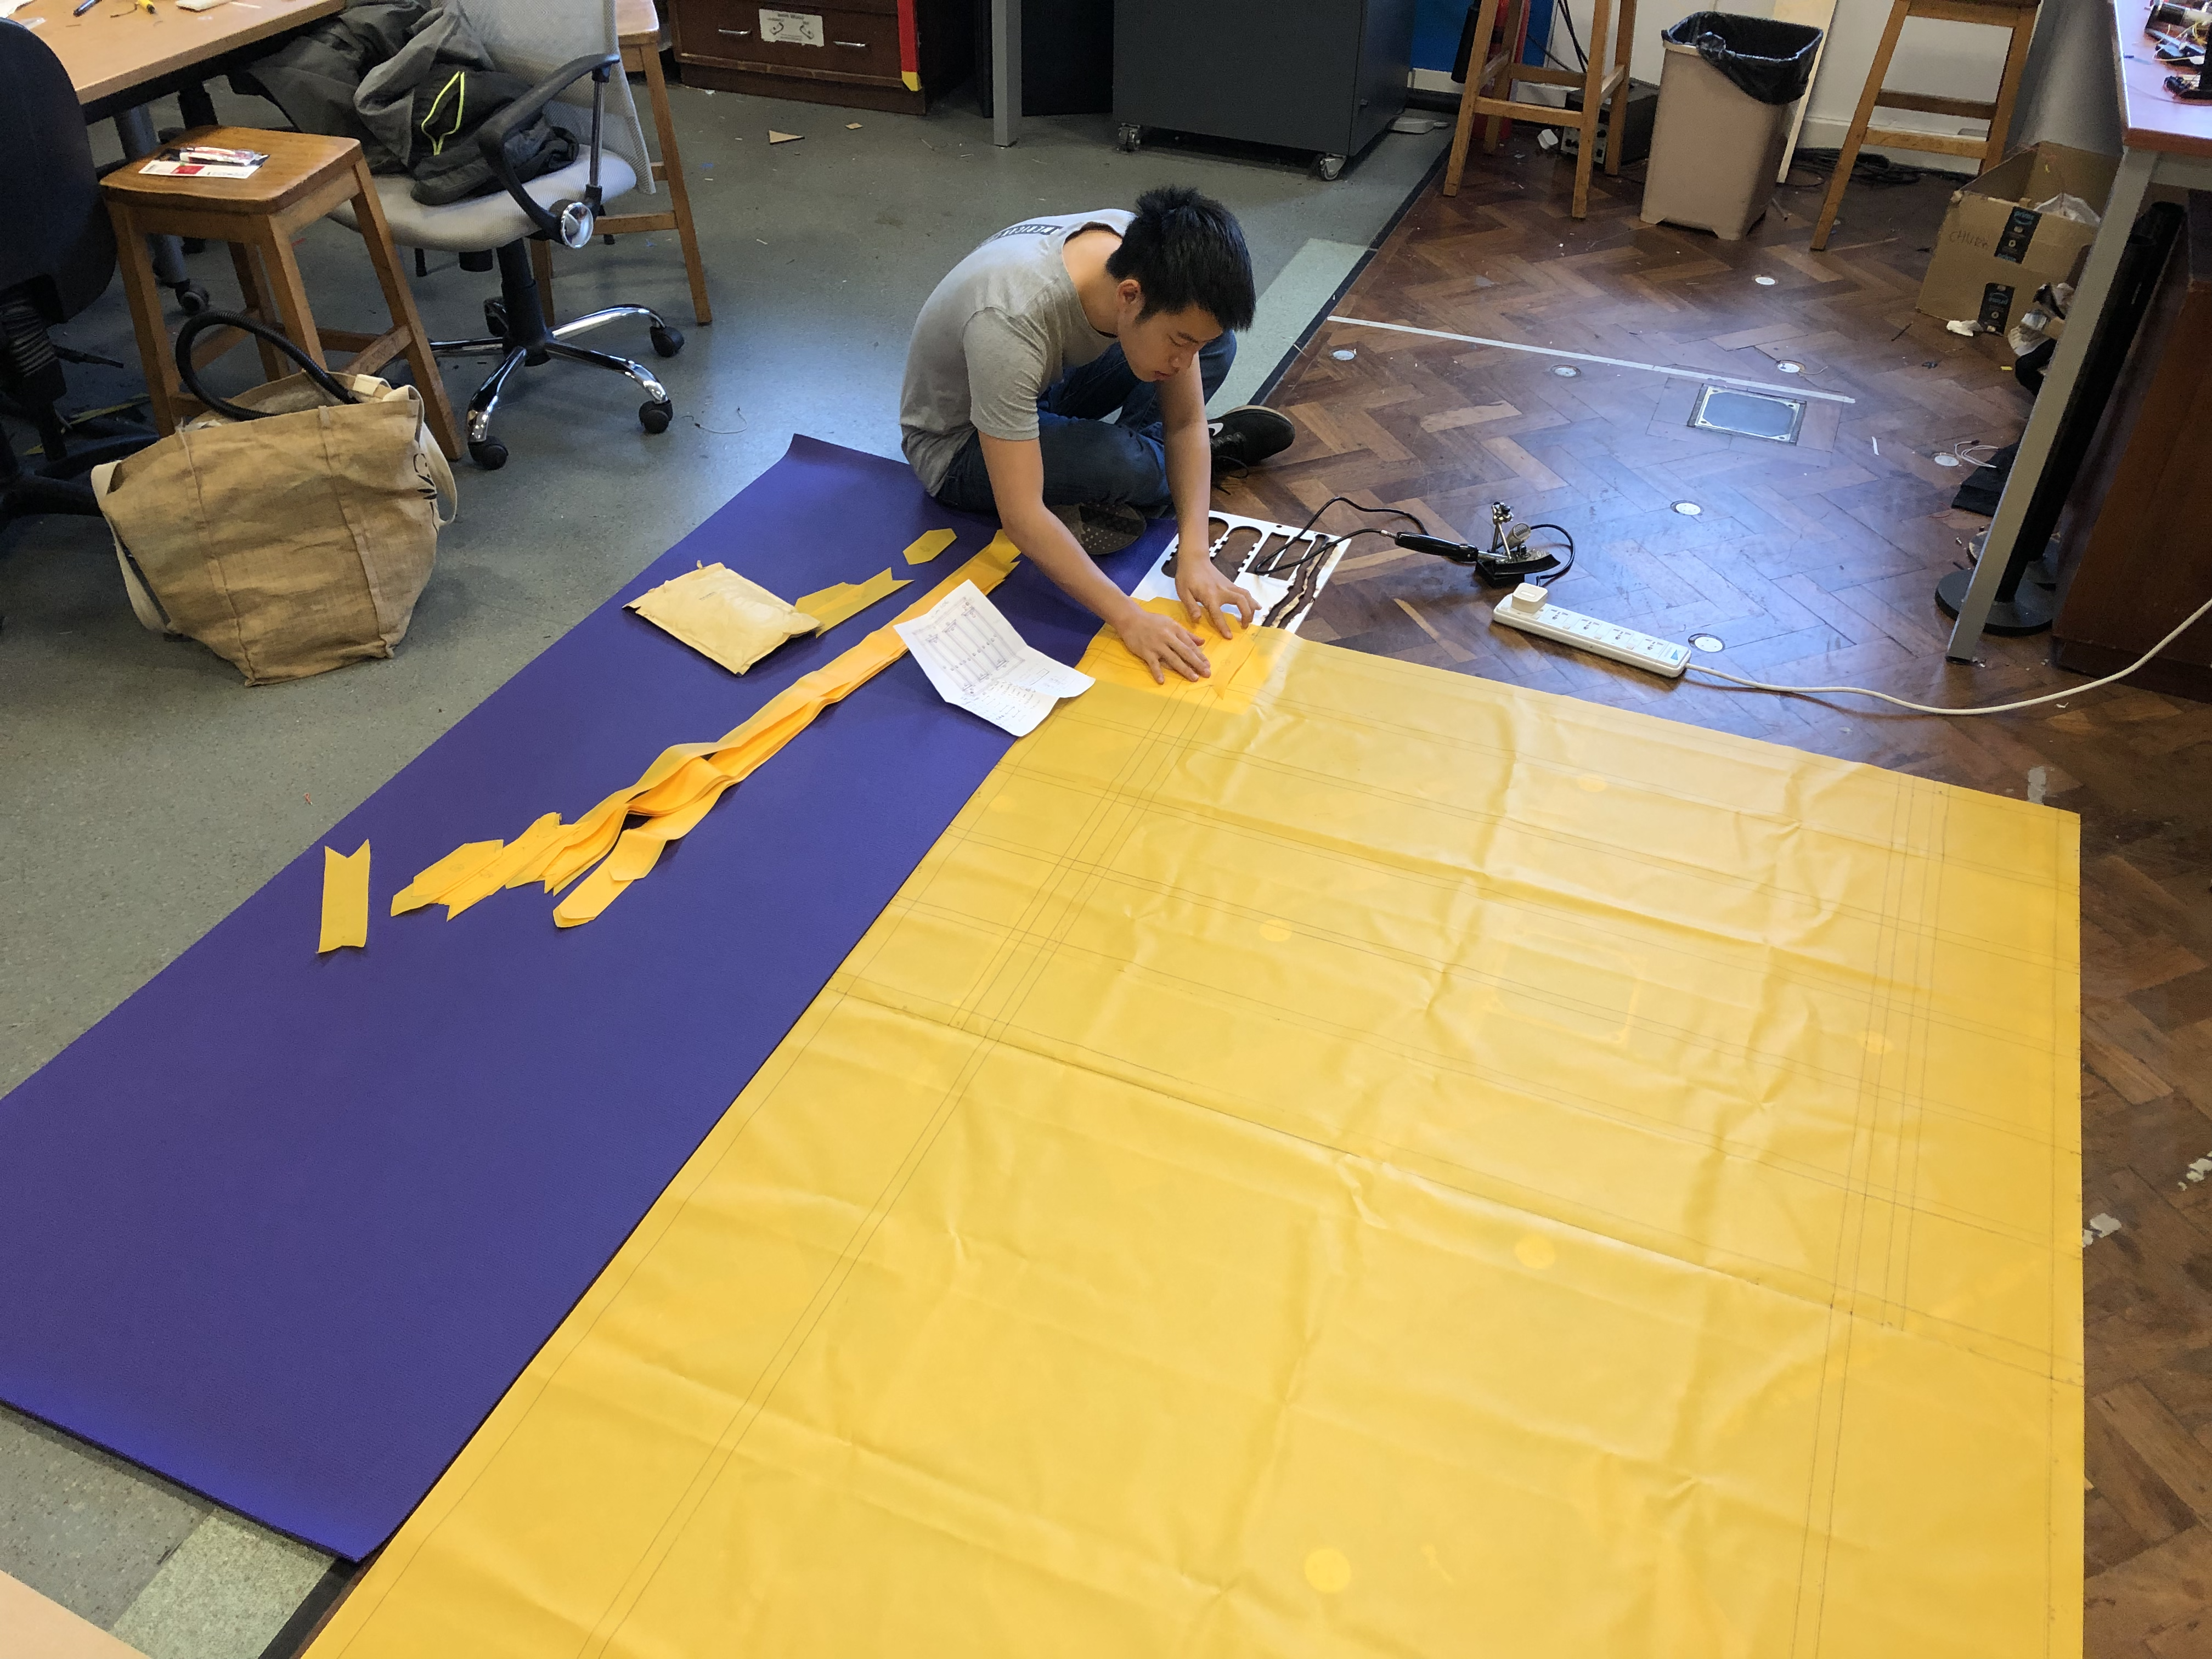
\includegraphics[height= 350, width=0.5\linewidth]{img/IMG_1081copy.png}
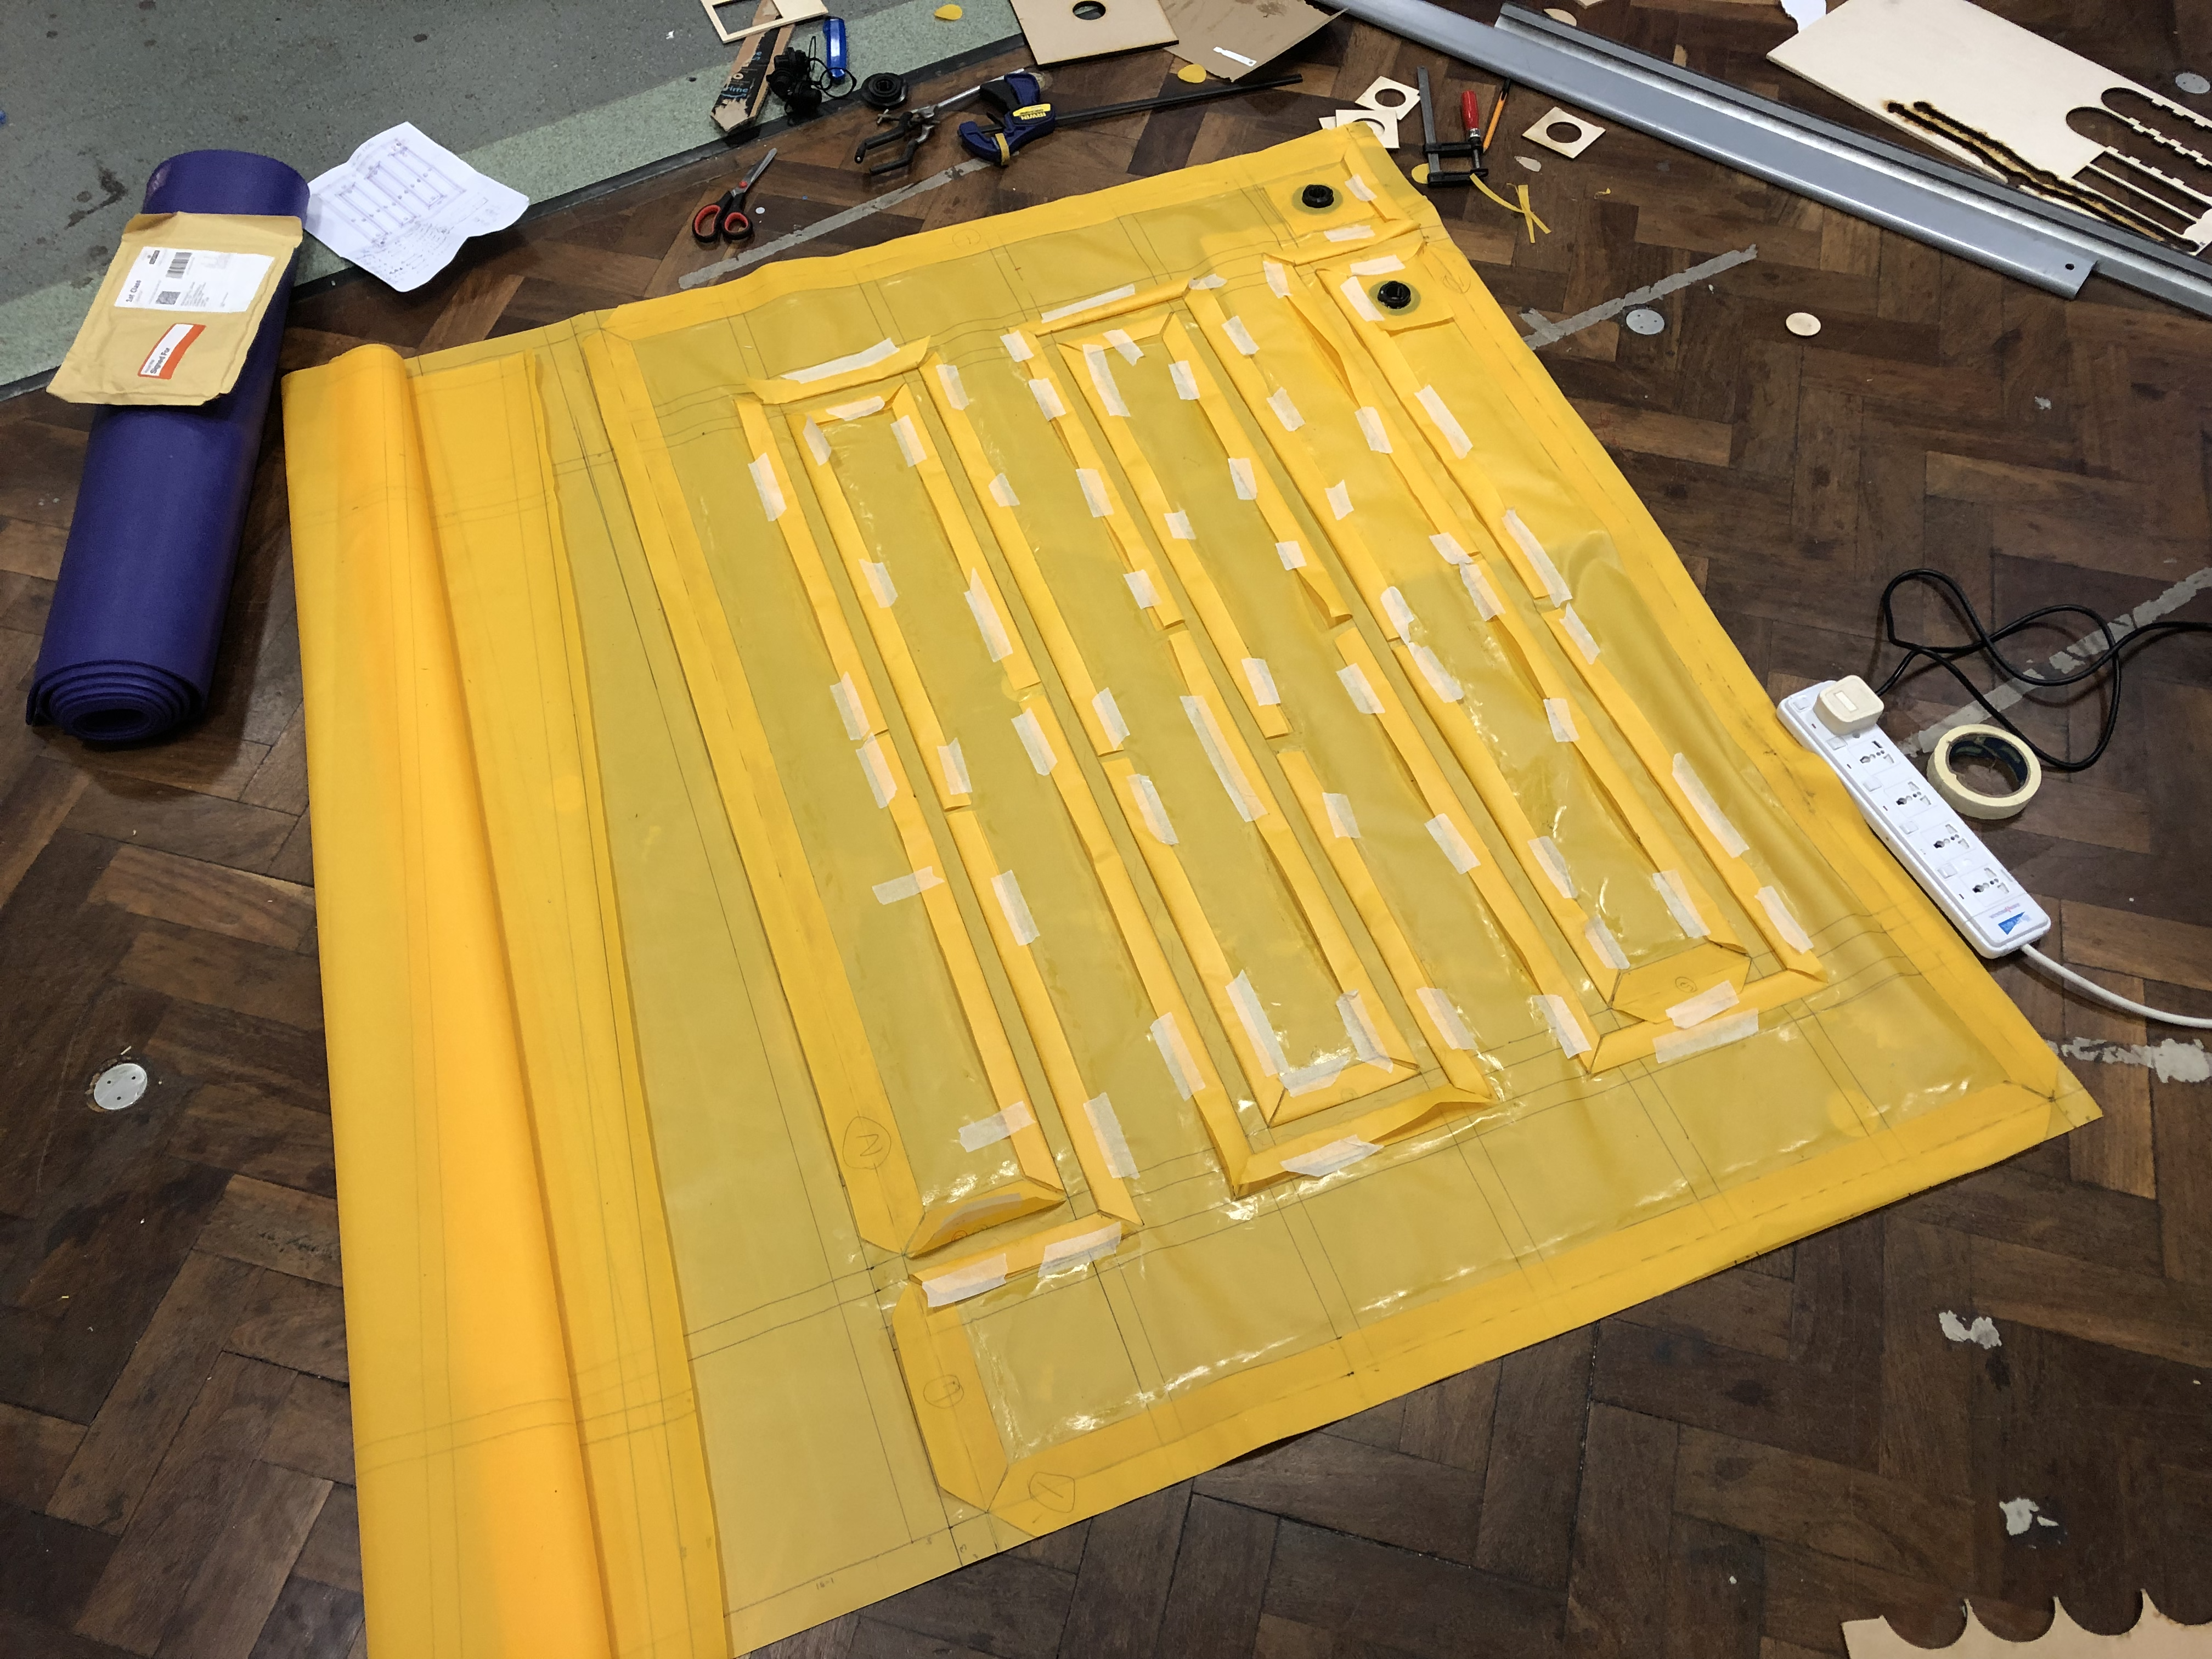
\includegraphics[height= 410, width=0.5\linewidth]{img/IMG_1097copy.png}
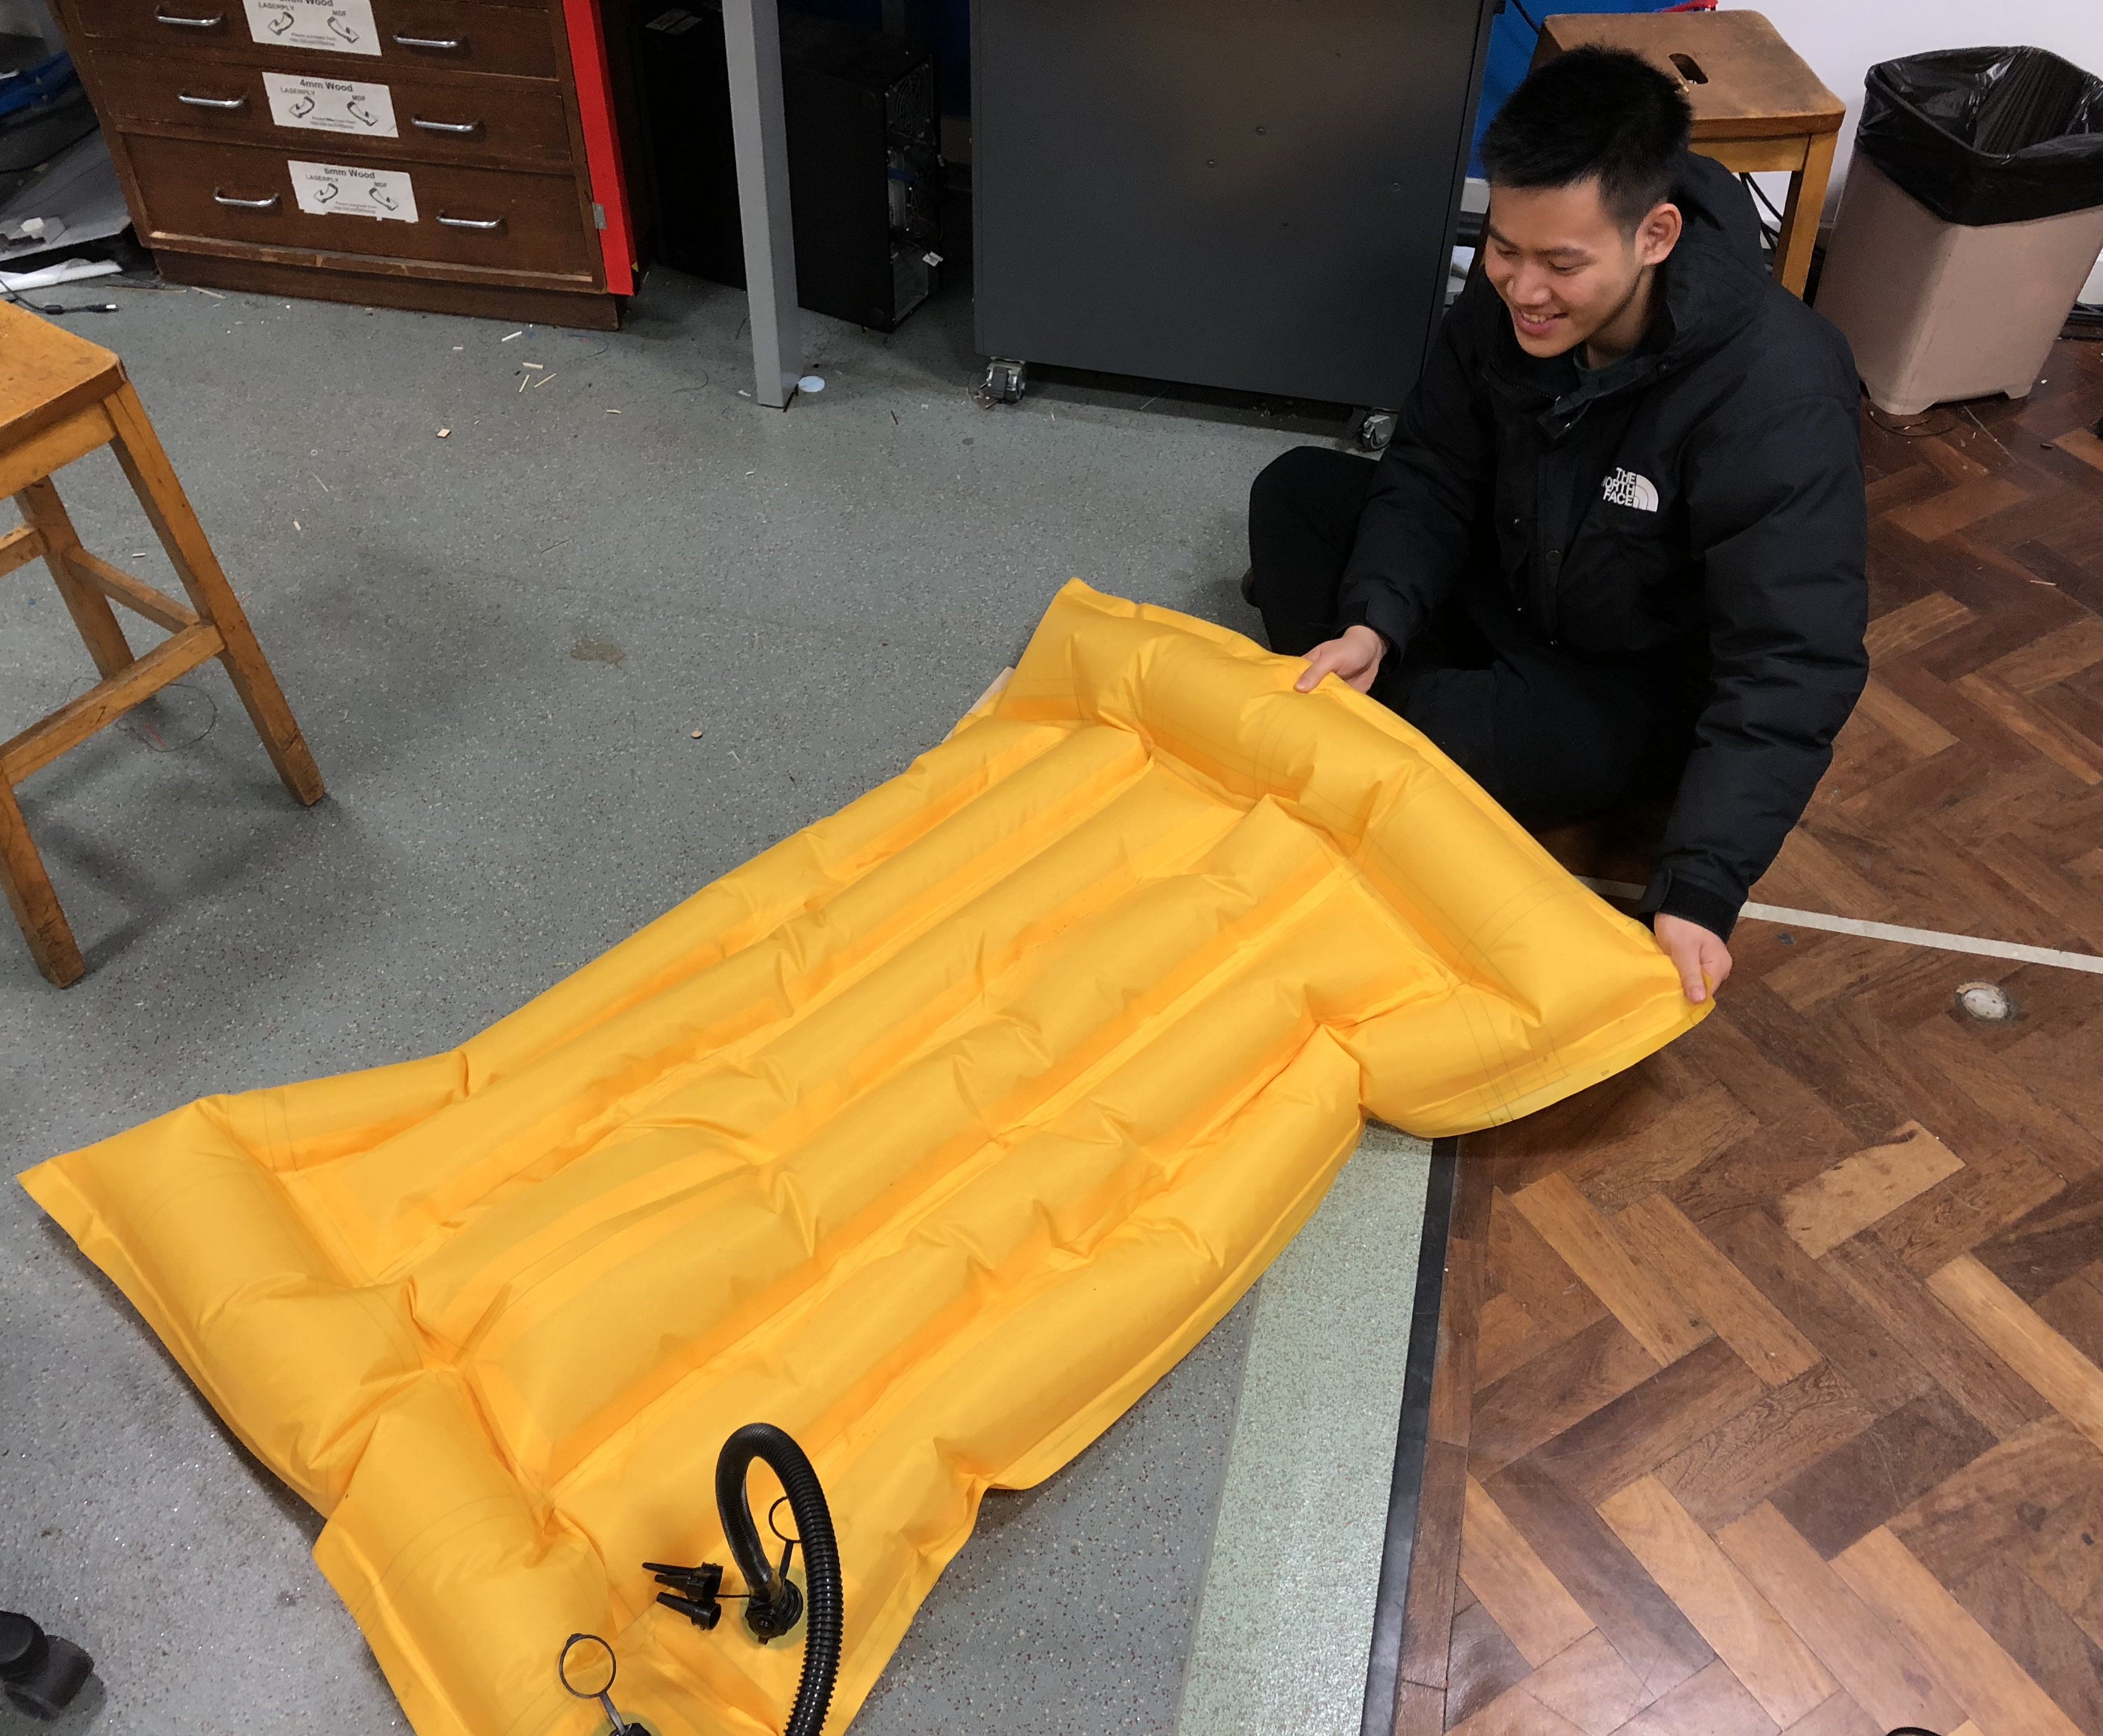
\includegraphics[height= 410, width=0.5\linewidth]{img/prototype.png}
\end{figure}


\end{block} 
%----------------------------------------------------------------------------------------

\begin{columns}[t,totalwidth=\twocolwid] % Split up the two columns wide column again

\begin{column}{\onecolwid} % The first column within column 2 (column 2.1)

%----------------------------------------------------------------------------------------
%	MATHEMATICAL SECTION
%----------------------------------------------------------------------------------------



%----------------------------------------------------------------------------------------

\end{column} % End of column 2.1
\begin{column}{\sepwid}\end{column} % Empty spacer column

\begin{column}{\onecolwid} % The second column within column 2 (column 2.2)

%----------------------------------------------------------------------------------------
%	RESULTS
%----------------------------------------------------------------------------------------


%----------------------------------------------------------------------------------------

\end{column} % End of column 2.2

\end{columns} % End of the split of column 2

\end{column} % End of the second column

\begin{column}{\sepwid}\end{column} % Empty spacer column

\begin{column}{\onecolwid} % The third column

%----------------------------------------------------------------------------------------
%	CONCLUSION
%----------------------------------------------------------------------------------------

\begin{block}{Pictogram Instructions}
\begin{figure}
\includegraphics[width=1\linewidth]{img/Instructions.pdf}
\end{figure}

\end{block}

%----------------------------------------------------------------------------------------
%	ADDITIONAL INFORMATION
%----------------------------------------------------------------------------------------
\begin{block}{SWOT analysis of our plan}
\textbf{STRENGTHS}
\begin{itemize}
\item Plan has involved physical prototyping and extensive research into existing products to find the most viable solutions 
\item Different strengths within the team that have been used together to formulate the plan
\end{itemize}
\textbf{WEAKNESSES }
\begin{itemize}
\item No first hand experience in the conditions of MSF locations and products that would be appropriate
\item Limited technology 
\end{itemize}
\textbf{OPPORTUNITIES }
\begin{itemize}
\item Producing mattresses to combat other commonly encountered problems
\end{itemize}
\textbf{THREATS }
\begin{itemize}
\item Failure to conduct clinical trials may mean the product may not actually be more useful than existing products 
\end{itemize}
\end{block}

%----------------------------------------------------------------------------------------
%	REFERENCES
%----------------------------------------------------------------------------------------

%----------------------------------------------------------------------------------------
%	ACKNOWLEDGEMENTS
%----------------------------------------------------------------------------------------

%\setbeamercolor{block title}{fg=black,bg=dblue!10} % Change the block title color

%\begin{block}{Acknowledgements}

%\small{\rmfamily{Nam mollis tristique neque eu luctus. Suspendisse rutrum congue nisi sed convallis. Aenean id neque dolor. Pellentesque habitant morbi tristique senectus et netus et malesuada fames ac turpis egestas.}} \\

%\end{block}

%----------------------------------------------------------------------------------------
%	CONTACT INFORMATION
%----------------------------------------------------------------------------------------
%\begin{block}{The Team}
%\begin{figure}
%\includegraphics[height= 275, width=0.75\linewidth]{img/team.png}
%\end{figure}
%\end{block}
%----------------------------------------------------------------------------------------

\end{column} % End of the third column

\begin{column}{\sepwid}\end{column} % Empty spacer column

\end{columns} % End of all the columns in the poster

\end{frame} % End of the enclosing frame
%\end{darkframes} % Uncomment for dark theme
\end{document}
